\documentclass[border=5pt]{standalone}
\usepackage{tikz}
\usetikzlibrary{positioning, arrows.meta, calc}

% Define Bayesian network styles with improved visual appearance
\tikzset{
  latent/.style={circle, draw, minimum size=1.2cm, thick},
  obs/.style={rectangle, draw, fill=gray!20, minimum size=1.2cm, thick},
  const/.style={circle, draw, fill=gray!20, minimum size=1.2cm, thick},
  det/.style={rectangle, draw, minimum size=1.2cm, thick}
}

% Define an improved plate function with more space around nodes
\newcommand{\drawplate}[3][]{%
  \draw[rounded corners=3pt, dashed, thick, #1] 
    ($(#2.north west)+(-0.25,0.25)$) rectangle 
    ($(#2.south east)+(0.25,-0.25)$);
  \node[anchor=north east] at ($(#2.south east)+(0.25,-0.25)$) {#3};
}

\begin{document}
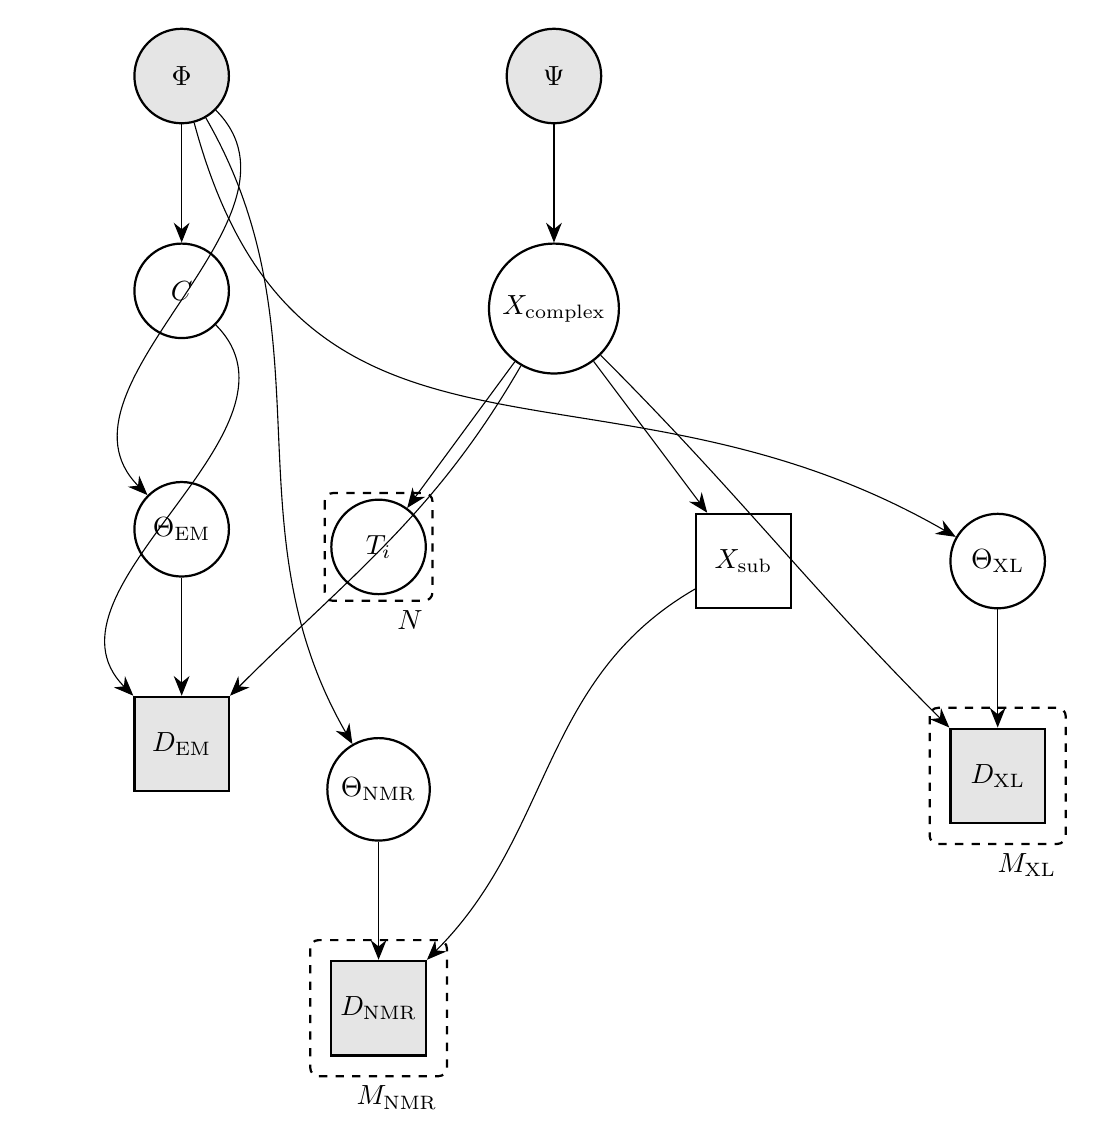
\begin{tikzpicture}[
  % Increased spacing for better clarity
  node distance=2.0cm and 2.5cm, 
  >={Stealth[length=2.5mm, width=2mm]},
  every node/.style={align=center, font=\sffamily}
]
  % LEVEL 1: Hyperparameters - well spaced at top
  \node[const] (Phi) {$\Phi$};
  \node[const, right=3.5cm of Phi] (Psi) {$\Psi$};

  % LEVEL 2: Global latent variables - aligned directly below their respective hyperparameters
  \node[latent, below=1.5cm of Phi] (C) {$C$};
  \node[latent, below=1.5cm of Psi] (Xcomplex) {$X_{\mathrm{complex}}$};

  % LEVEL 3: Subsystems & nuisance parameters - proper horizontal spacing
  % Left branch
  \node[latent, below=1.8cm of C] (ThetaEM) {$\Theta_{\mathrm{EM}}$};
  
  % Middle-left branch
  \node[latent, below left=2cm and 1.2cm of Xcomplex] (Ti) {$T_i$};
  \node[latent, below=1.8cm of Ti] (ThetaNMR) {$\Theta_{\mathrm{NMR}}$};
  
  % Middle-right branch
  \node[det, below right=2cm and 1.2cm of Xcomplex] (Xsub) {$X_{\mathrm{sub}}$};
  
  % Right branch
  \node[latent, right=2cm of Xsub] (ThetaXL) {$\Theta_{\mathrm{XL}}$};

  % LEVEL 4: Observed data - aligned directly below their respective parameters
  \node[obs, below=1.5cm of ThetaEM] (DEM) {$D_{\mathrm{EM}}$};
  \node[obs, below=1.5cm of ThetaNMR] (DNMR) {$D_{\mathrm{NMR}}$};
  \node[obs, below=1.5cm of ThetaXL] (DXL) {$D_{\mathrm{XL}}$};

  % Edges with improved routing to avoid crossings
  % Hyperparameter influences
  \draw[->] (Phi) -- (C);
  \draw[->] (Phi) to[out=-45, in=135] (ThetaEM);
  \draw[->] (Phi) to[out=-60, in=120] (ThetaNMR);
  \draw[->] (Phi) to[out=-75, in=150, looseness=1.2] (ThetaXL);
  \draw[->] (Psi) -- (Xcomplex);
  
  % Structure influences
  \draw[->] (Xcomplex) -- (Ti);
  \draw[->] (Xcomplex) -- (Xsub);
  
  % EM data pathway
  \draw[->] (C) to[out=-45, in=135] (DEM);
  \draw[->] (Xcomplex) to[out=-120, in=45] (DEM);
  \draw[->] (ThetaEM) -- (DEM);
  
  % NMR data pathway
  \draw[->] (Xsub) to[out=-150, in=45] (DNMR);
  \draw[->] (ThetaNMR) -- (DNMR);
  
  % XL data pathway
  \draw[->] (Xcomplex) to[out=-45, in=135] (DXL);
  \draw[->] (ThetaXL) -- (DXL);

  % Draw plates with improved spacing
  \drawplate{Ti}{$N$}
  \drawplate{DNMR}{$M_{\mathrm{NMR}}$}
  \drawplate{DXL}{$M_{\mathrm{XL}}$}

\end{tikzpicture}
\end{document}